\documentclass{article}
\usepackage[utf8]{inputenc}

\title{Ph20 HW3}
\author{Nathan T Barton }
\date{February 8, 2019}

\usepackage{natbib}
\usepackage{graphicx}

\begin{document}

\maketitle

\section{Introduction}
During this week, I wrote a python program to investigate numerical techniques for solving differential equations, as applied to the simple harmonic oscillator system.  The code for the main program is hw3.ipynb, which defines functions for each of the numerical techniques implemented, and generates the corresponding figures.  

The Euler methods were implemented using numpy arrays and matrices, so that each time-step could be computed as the product of the previous time-step and a time-step matrix.  This made the code efficient and easy to modify to implement the various methods.  In order to directly compare the methods, all methods were called with the same parameters, notably with $x_0 = 1$, $v_0 = 0$, a max time of $t_{max} = 25$, and time-step $h = 0.05$

\newpage

\section{Results}

\subsection{Explicit Euler Method}

\begin{figure}[h!]
\centering
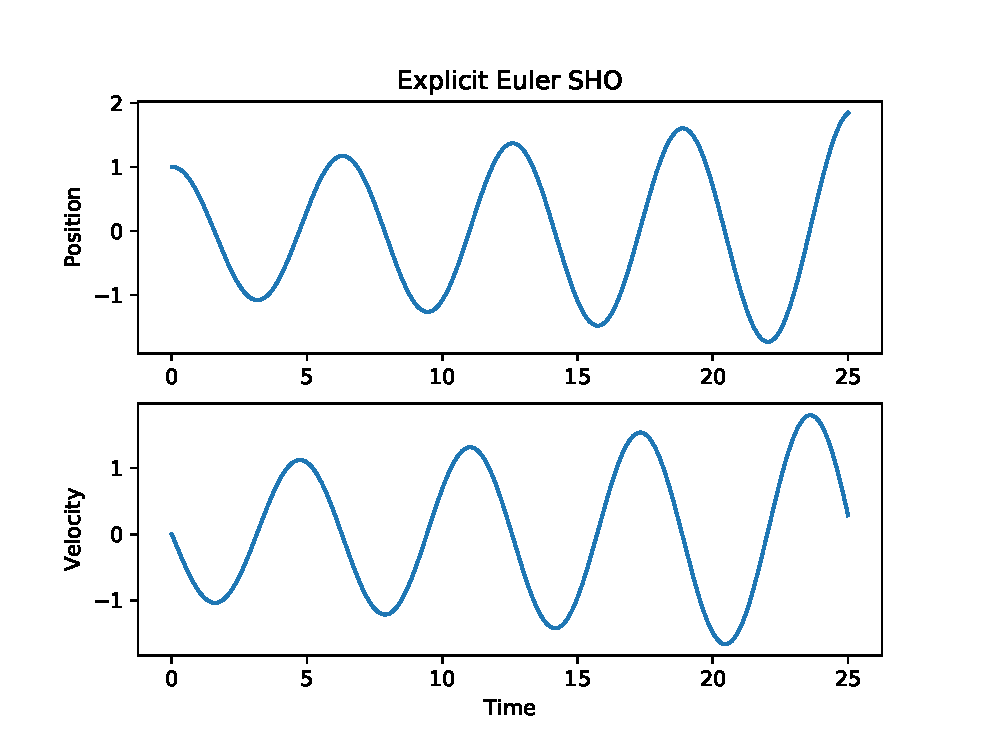
\includegraphics[scale=.75]{fig/explicit_plot.eps}
\caption{Oscillations of a SHO using the Explicit Euler Method}
\label{fig:exp_plot}
\end{figure}

In Figure \ref{fig:exp_plot}, we can see sinusoidal-like oscillations of position and velocity for the explicit Euler method.  However, we can notice a slight increasing trend in amplitude, as the errors accumulate.

\newpage

\begin{figure}[h!]
\centering
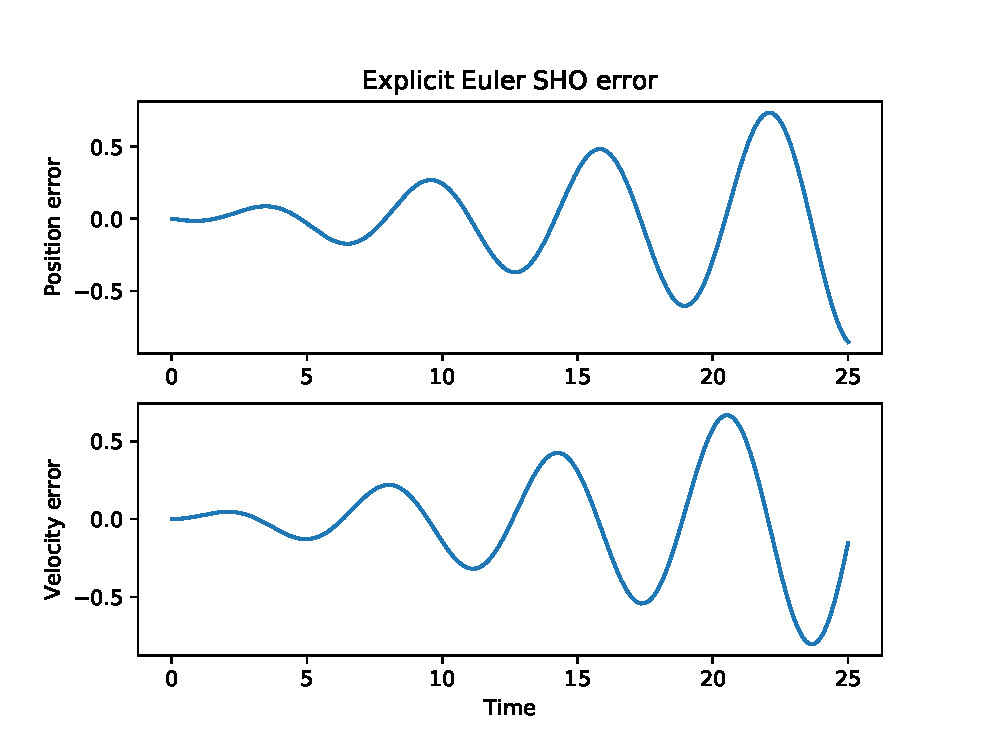
\includegraphics[scale=.75]{fig/explicit_error.eps}
\caption{Error of SHO using Explicit Euler Method}
\label{fig:exp_error}
\end{figure}

To better show the trend in error, in Figure \ref{fig:exp_error}, the error in the position and velocity of the oscillator is plotted over time.  The error was computed first by computing the analytic solution for the harmonic oscillator, and finding the difference between the expected analytic value and the numerically computed value.  Here, we can see that the error reaches local maxima with each crest/trough of the oscillator waveform.  The error directly out of phase with the oscillator, and steadily grows with time.  

\newpage

\begin{figure}[h!]
\centering
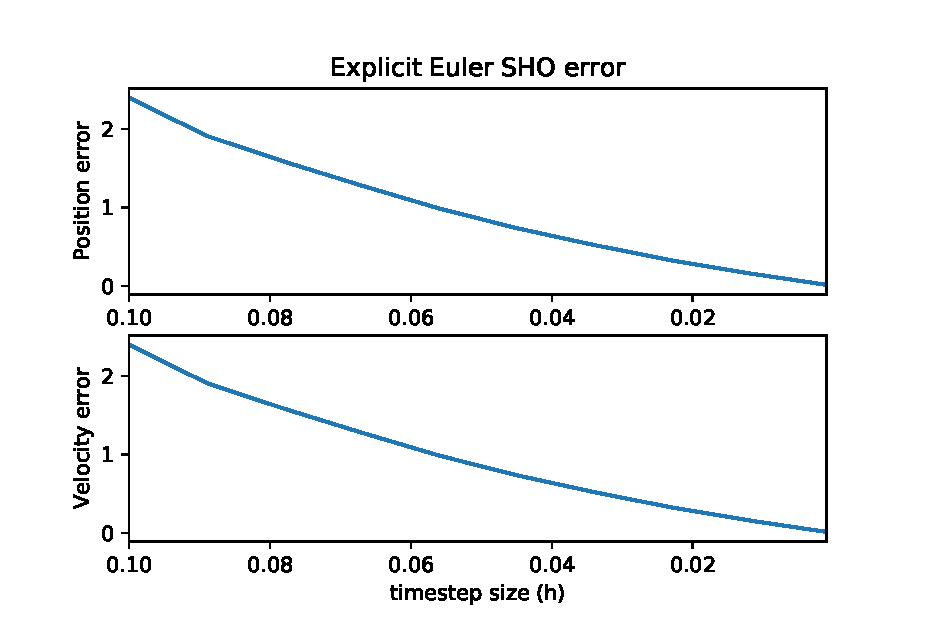
\includegraphics[scale=0.75]{fig/explicit_error_vs_h.eps}
\caption{Maximum error of Explicit Euler SHO over 25 oscillations versus time-step size}
\label{fig:exp_error_h}
\end{figure}

Next, I compared the error of the Explicit Euler SHO for varying time-step values in order to see the truncation error.  In Figure \ref{fig:exp_error_h}, we see that, for small values of $h$, the error decrease is roughly linearly proportional to the time-step size

\newpage

\begin{figure}[h!]
\centering
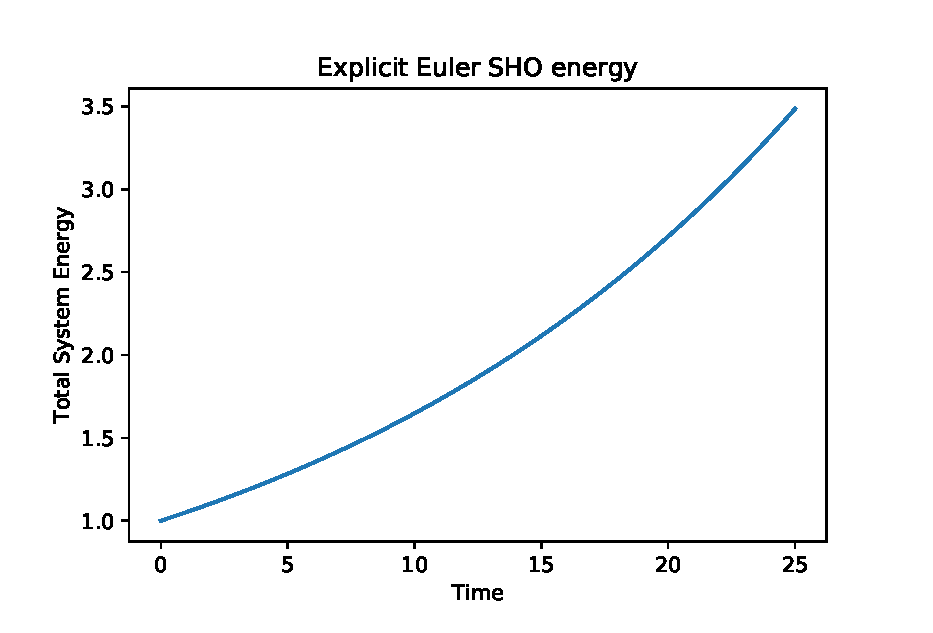
\includegraphics[scale=0.75]{fig/explicit_energy.eps}
\caption{Energy of Explicit Euler SHO over time}
\label{fig:exp_energy}
\end{figure}

In Figure \ref{fig:exp_energy}, we see that the energy of the system, as modelled by the Explicit Euler method, increases roughly exponentially with time.  This is expected from the increasing amplitude as seen in figure \ref{fig:exp_plot}, and would limit the utility of the method for accurately modelling the amplitude of the system over long time scales.  

\newpage

\subsection{Implicit Euler Method}

\begin{figure}[h!]
\centering
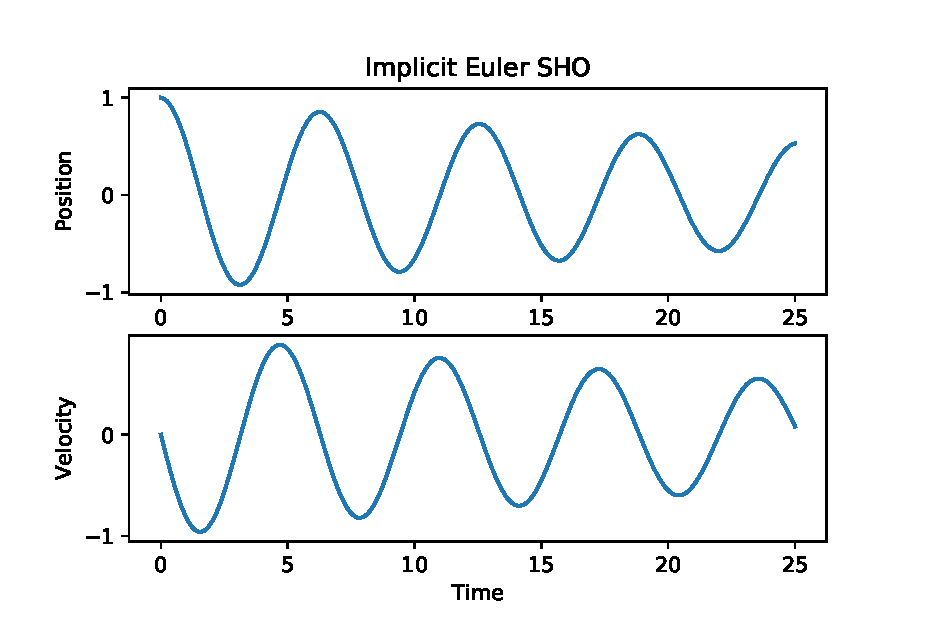
\includegraphics[scale=.75]{fig/implicit_plot.eps}
\caption{Oscillations of a SHO using the Implicit Euler Method}
\label{fig:imp_plot}
\end{figure}

In Figure \ref{fig:imp_plot}, as with the Explicit Euler method, we can see sinusoidal-like oscillations of position and velocity for the implicit Euler method.  However, unlike with the Explicit method, we can notice a slight decreasing trend in amplitude.  

\newpage

\begin{figure}[h!]
\centering
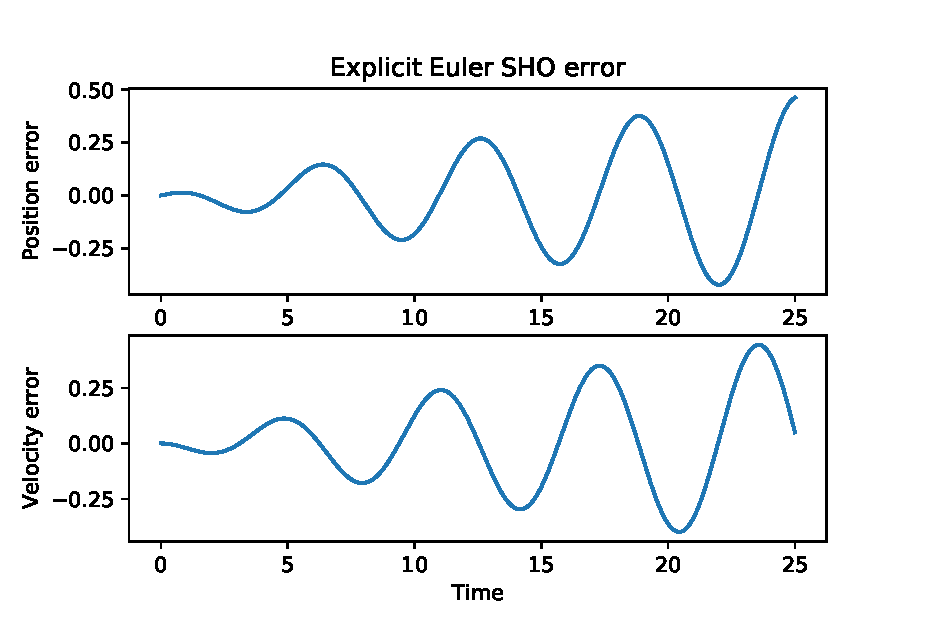
\includegraphics[scale=.75]{fig/implicit_error.eps}
\caption{Error of SHO using Implicit Euler Method}
\label{fig:imp_error}
\end{figure}

Figure \ref{fig:imp_error} shows the error in the position and velocity of the oscillator over time.  Similar to the Explicit method, we can see that the error reaches local maxima with each crest/trough of the oscillator waveform.  However, in this case, the error is in phase with the oscillator, and steadily grows with time, resulting in a decreasing amplitude over time.  

\newpage

\begin{figure}[h!]
\centering
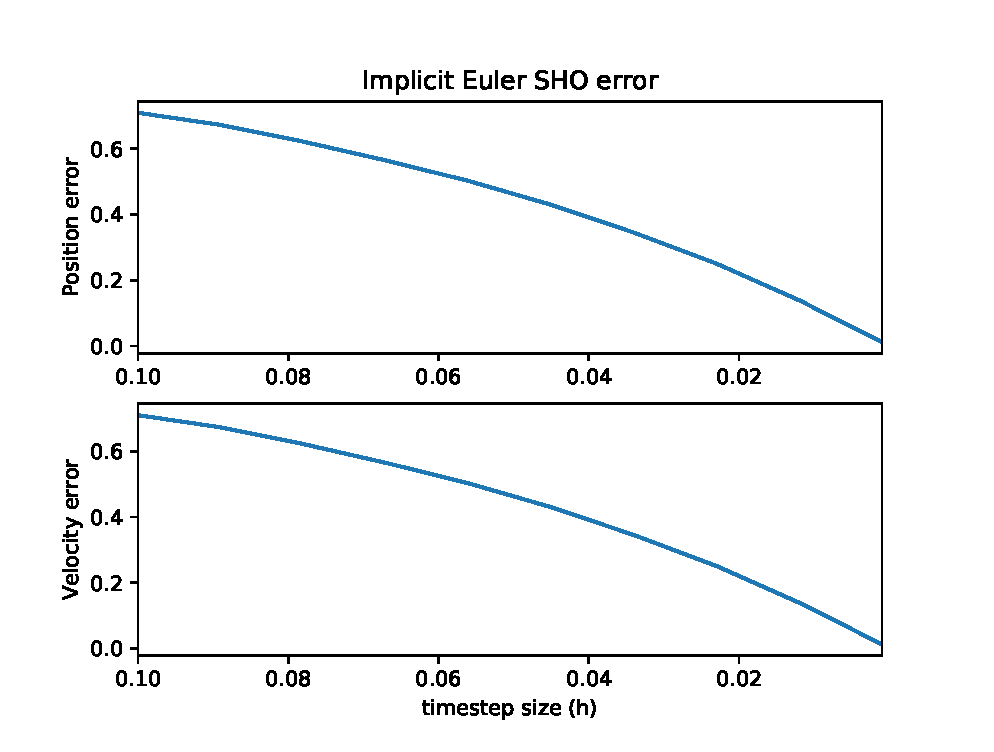
\includegraphics[scale=0.75]{fig/implicit_error_vs_h.eps}
\caption{Maximum error of Implicit Euler SHO over 25 oscillations versus time-step size}
\label{fig:imp_error_h}
\end{figure}

Figure \ref{fig:exp_error_h} shows the truncation error for the implicit Euler method.  Once again, we see that, for small values of $h$, the error decrease is roughly linearly proportional to the time-step size.  However, unlike the Explicit method, the truncation error is concave downwards with decreasing time-step size, and thus will scale better with increasing precision.  

\newpage

\begin{figure}[h!]
\centering
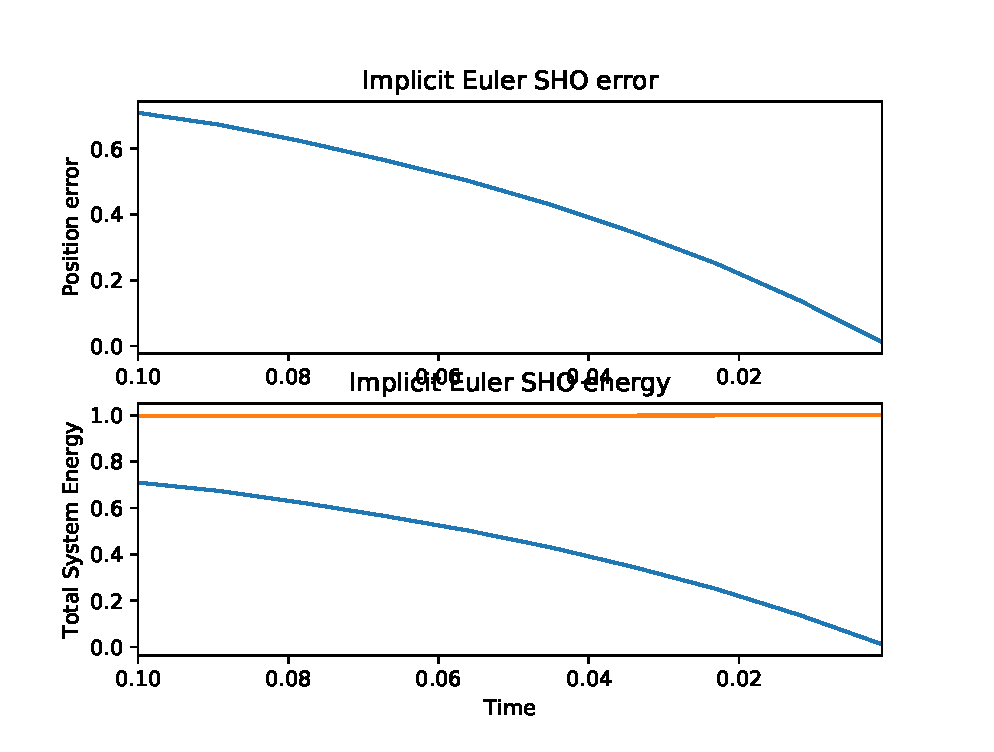
\includegraphics[scale=0.75]{fig/implicit_energy.eps}
\caption{Energy of implicit Euler SHO over time}
\label{fig:imp_energy}
\end{figure}

Figure \ref{fig:imp_energy} shows that the energy of the system, as modelled by the Implicit Euler method, decreases roughly exponentially with time.  This is expected from the decreasing amplitude as seen in figure \ref{fig:imp_plot}, and once again would limit the utility of the method for accurately modelling the amplitude of the system over long time scales.  

\newpage

\subsection{Phase-space of Euler methods and Symplectic Method}

\begin{figure}[h!]
\centering
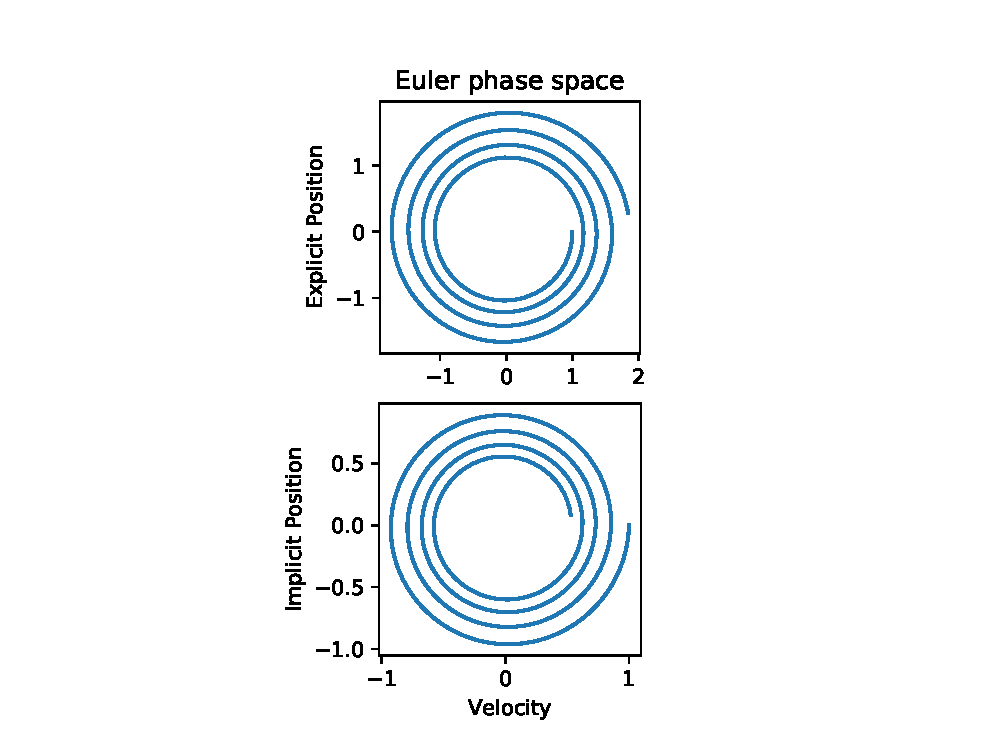
\includegraphics[scale=0.75]{fig/exp_imp_phase.eps}
\caption{phase-space plot for Explicit and Implicit Euler SHO}
\label{fig:exp_imp_phase}
\end{figure}

Figure \ref{fig:exp_imp_phase} shows the phase space plot for the Explicit and Implicit Euler methods.  We can see that the Explicit method spirals outward, while the Implicit method spirals inwards as a result of the increasing/decreasing energies of the modeled systems respectively.  

\newpage 

In order to reduce this energy error, I implemented the Symplectic Euler method.  In Figure \ref{fig:sym_phase}, we can see that, indeed, the phase space plot produces a closed curve, and thus energy error is conserved in this model.  

\begin{figure}[h!]
\centering
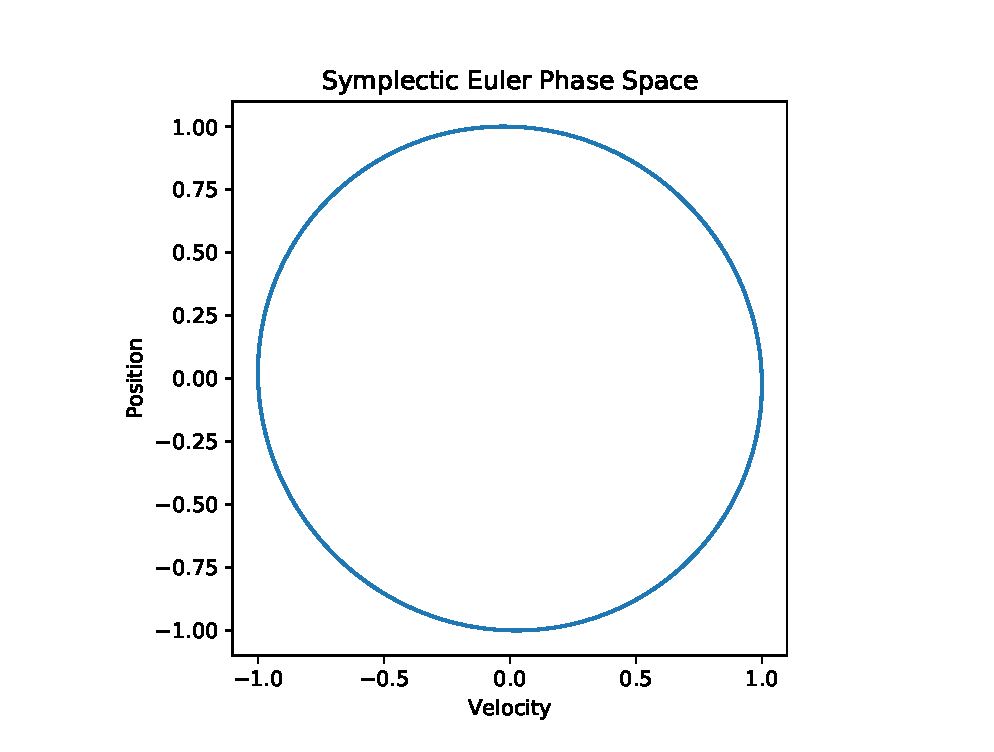
\includegraphics[scale=0.75]{fig/symplectic_phase_plot.eps}
\caption{phase-space plot for Symplectic Euler SHO}
\label{fig:sym_phase}
\end{figure}

\newpage

\begin{figure}[h!]
\centering
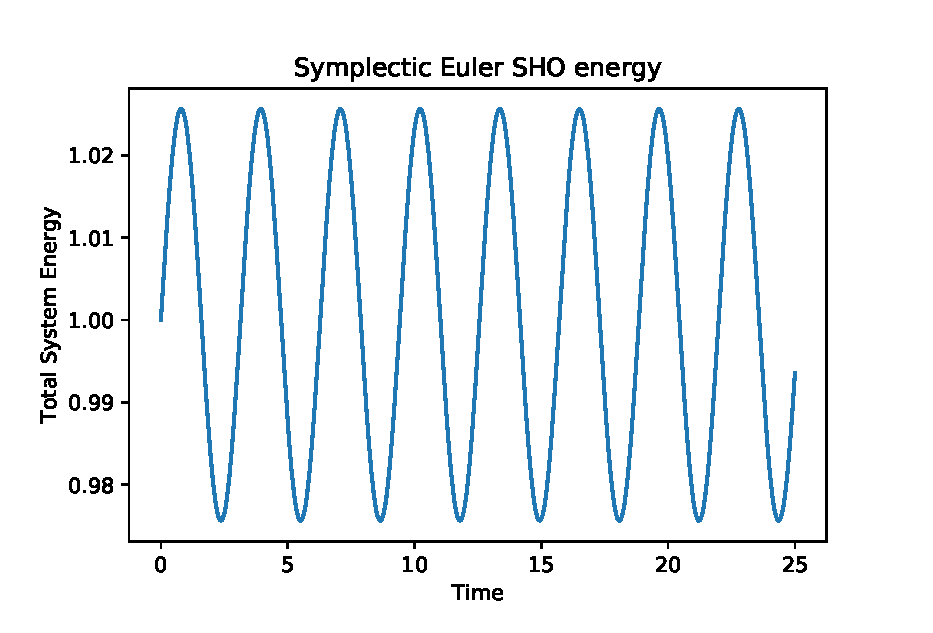
\includegraphics[scale=0.75]{fig/symplectic_energy.eps}
\caption{Energy plot for Symplectic Euler SHO}
\label{fig:sym_energy}
\end{figure}

In Figure \ref{fig:sym_energy}, we can see that the error in energy for the system oscillates with time, yet remains bounded.  Therefore, the error in the amplitude, and thus energy of the system, will not grow over long timescales.  

\newpage

To study the other sources of error with the Symplectic method, in Figure \ref{fig:sym_plot}, the position and velocity is plotted out to time $t_{max} = 10000$.  Here, we can see that the energy/amplitude of the system is modelled correctly, however the Symplectic method introduces a phase shift error.  Thus, while the Symplectic method preserves energy conservation, the method would be ill-suited to situations where the phase of the system needs to be modelled properly over long timescales.  

\begin{figure}[h!]
\centering
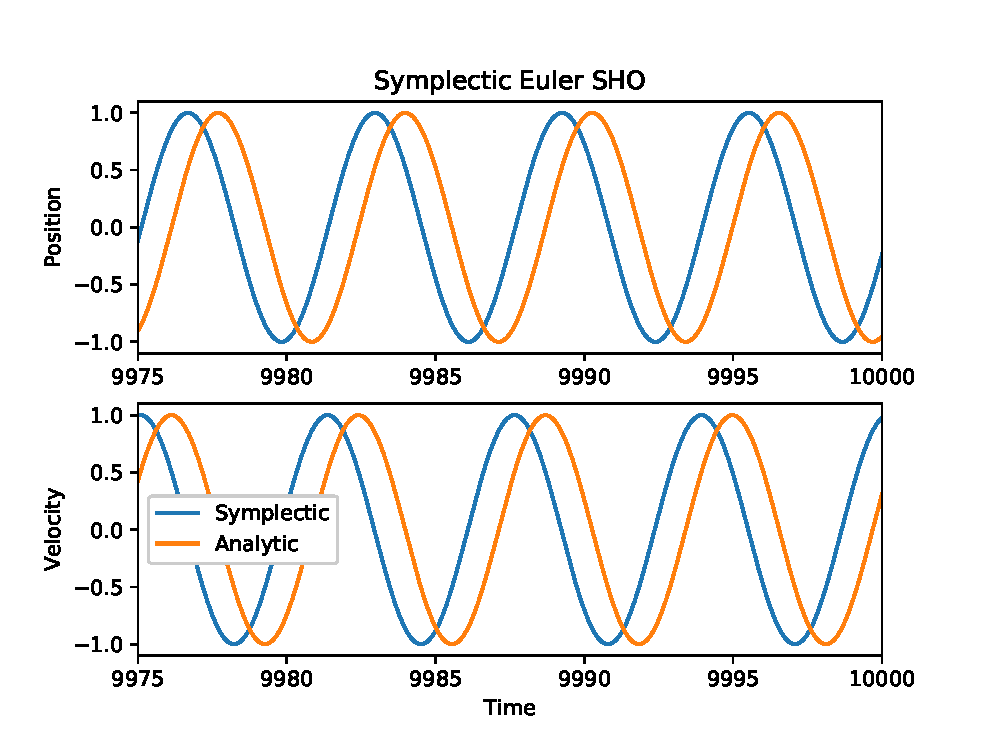
\includegraphics[scale=0.75]{fig/symplectic_plot.eps}
\caption{phase error of Symplectic Euler SHO}
\label{fig:sym_plot}
\end{figure}

\section{Conclusion}
Overall, we can see that each of these first-order methods can model and preserve different aspects of the simple harmonic oscillator system.  The suitability of each method for a given application would depend on the tolerance for different types of error (energy vs phase, etc).  

\end{document}
